\documentclass[../main.tex]{subfiles}

\begin{document}
	

\section{Access Control Container Metadata}

Containers may require some primitives, either provided by the system or by other containers. To our knowledge, no existing runtime container service manage the access rights of container over the primitives it requires. We propose to solve this issue by adding some metadata to the container in order to configure a policy enforcement module within the Runtime Containers Service, as specified in deliverable D4.1.1 \cite{TinyPART-d411}.\\

As depicted in figure \ref{fig:metadata}, the metadata consists in the following fields:
\begin{itemize}
	\item a container description which contains a uid identifying the container, the type of container (e.g. rbpf, wasm, ...) and a signed token which contains the list of system calls authorized for this container.
	\item a list of endpoints (e.g. another container, a local resource such as a specific bus or a remote resource) characterized by an ID, a type and a signed token, called authorization code, that lists which endpoint functions are authorized to be used by the current container. As illustrated with the fields "...", the structure is flexible enough to add an unfixed number of fields to describe the endpoint,
	\item some security-related information such as various checksums or the container lifetime. We also reserved a field called vendor\_secu for security data specific to the container provider. This could for example be a key to be stored in a cryptographic module or a reference to a key stored in a cryptographic module that the container could use during its lifetime.  
\end{itemize}  

\task{}{Samuel}{Comment tu fais pour permettre d'ajouter un nombre non défini d'éléments dans les différentes structures ? il y a un séparateur ? ou alors tu as des clés/valeurs comme en json ? }

\begin{figure}[hbt!]
	\centering
	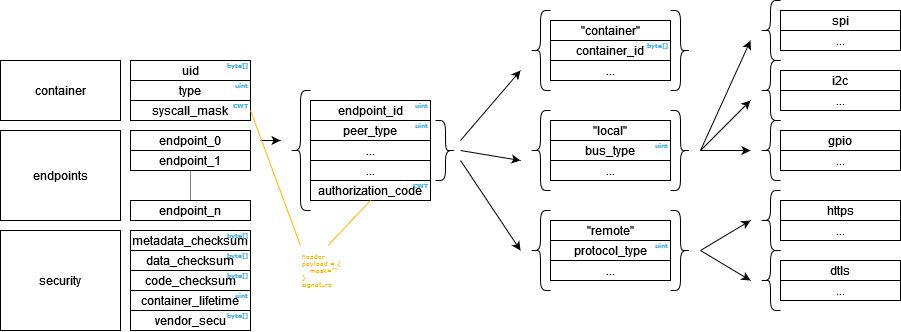
\includegraphics[width=\linewidth]{images/metadata.png}
	\caption{Container Metadata}
	\label{fig:metadata}
\end{figure}

\end{document}
